\begin{figure}[H]
    \renewcommand{\figurename}{Рисунок}
    \centering{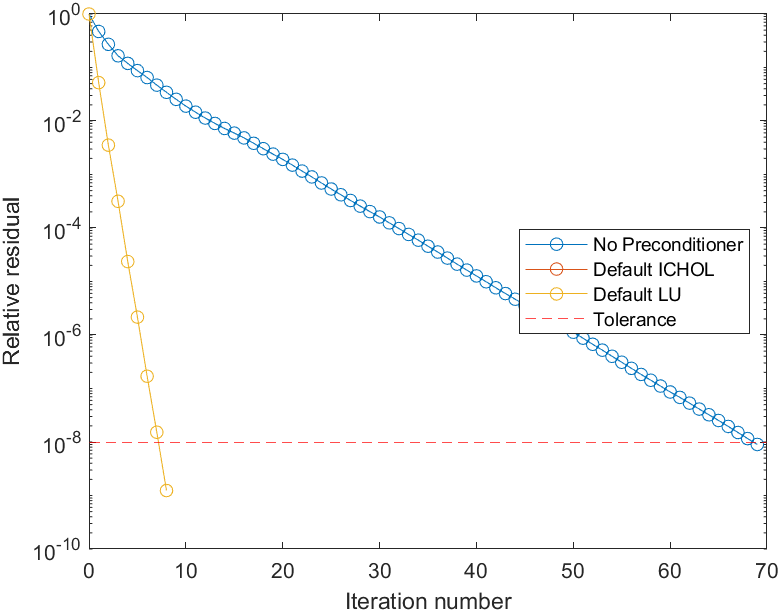
\includegraphics[scale=0.70]{img/thermomech/bicg}}
    \caption{История невязок методом bicg для матрицы Thermomech_dM}
    \label{fig:image_23}
\end{figure}

\begin{figure}[H]
    \renewcommand{\figurename}{Рисунок}
    \centering{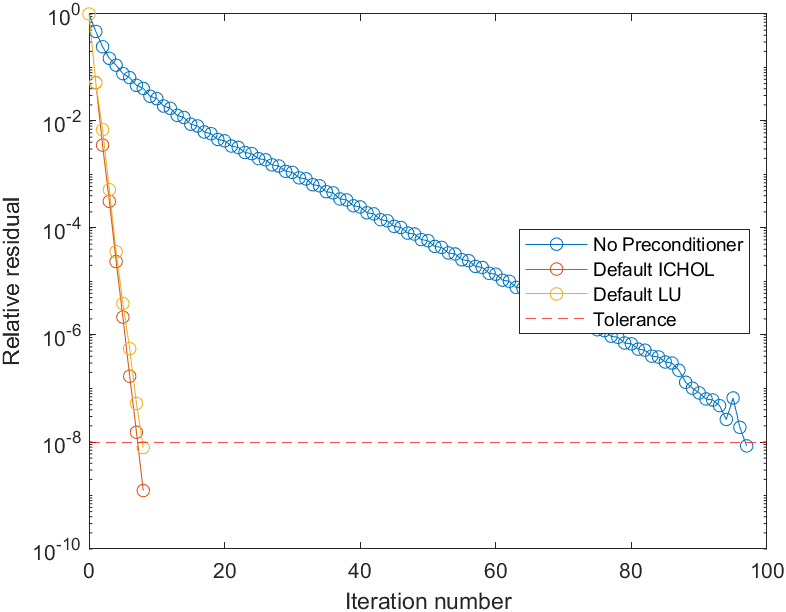
\includegraphics[scale=0.70]{img/thermomech/bicgstab}}
    \caption{История невязок методом bicgstab для матрицы Thermomech_dM}
    \label{fig:image_24}
\end{figure}

\begin{figure}[H]
    \renewcommand{\figurename}{Рисунок}
    \centering{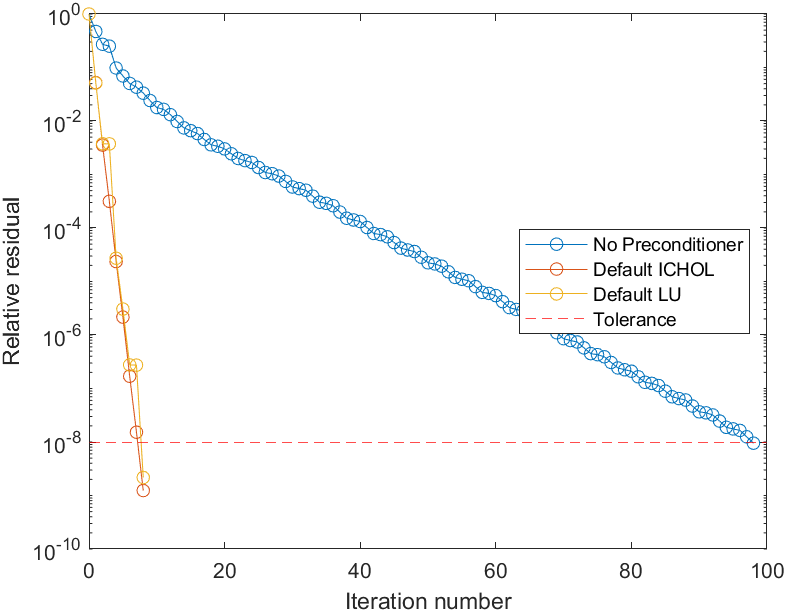
\includegraphics[scale=0.70]{img/thermomech/bicgstabl}}
    \caption{История невязок методом bicgstabl для матрицы Thermomech_dM}
    \label{fig:image_25}
\end{figure}

\begin{figure}[H]
    \renewcommand{\figurename}{Рисунок}
    \centering{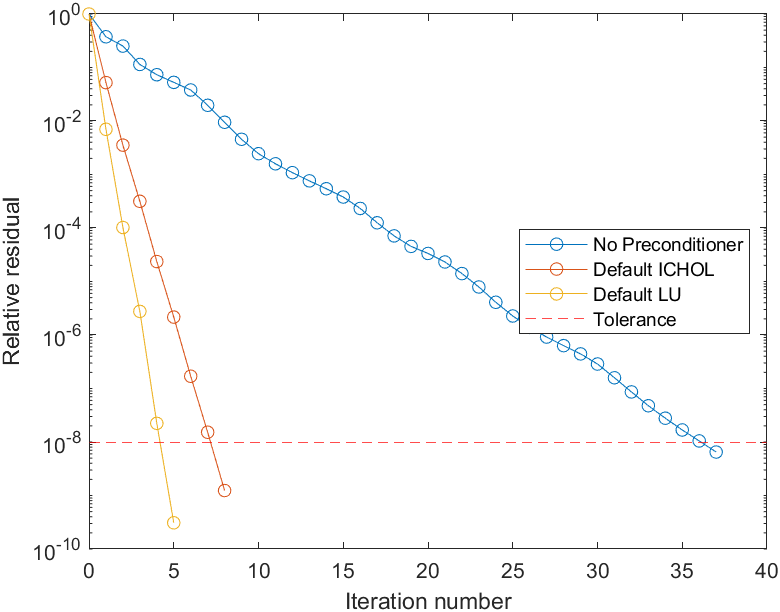
\includegraphics[scale=0.70]{img/thermomech/cgs}}
    \caption{История невязок методом cgs для матрицы Thermomech_dM}
    \label{fig:image_26}
\end{figure}

\begin{figure}[H]
    \renewcommand{\figurename}{Рисунок}
    \centering{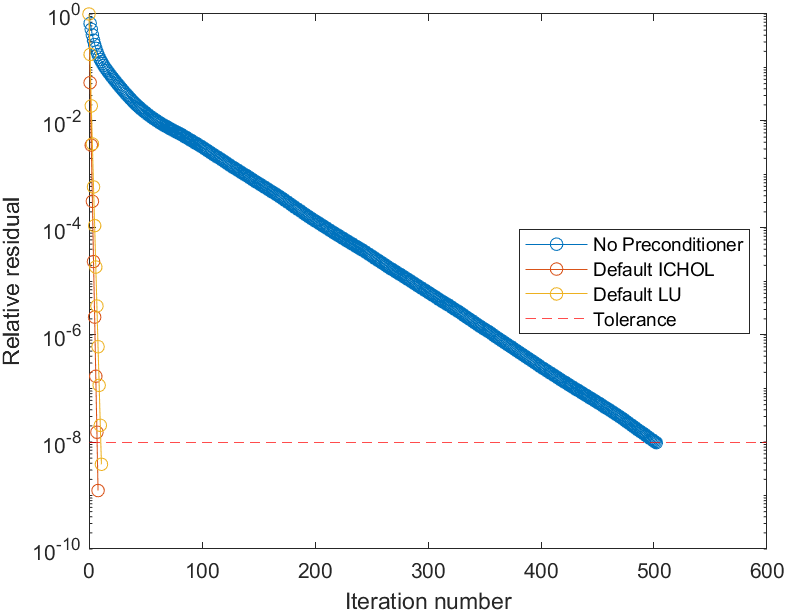
\includegraphics[scale=0.70]{img/thermomech/lsqr}}
    \caption{История невязок методом lsqr для матрицы Thermomech_dM}
    \label{fig:image_27}
\end{figure}

\begin{figure}[H]
    \renewcommand{\figurename}{Рисунок}
    \centering{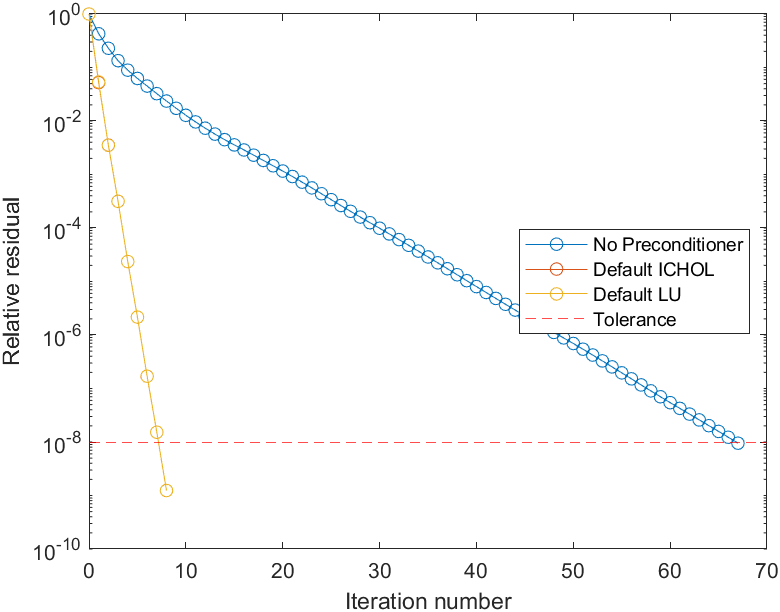
\includegraphics[scale=0.70]{img/thermomech/minres}}
    \caption{История невязок методом minres для матрицы Thermomech_dM}
    \label{fig:image_28}
\end{figure}

\begin{figure}[H]
    \renewcommand{\figurename}{Рисунок}
    \centering{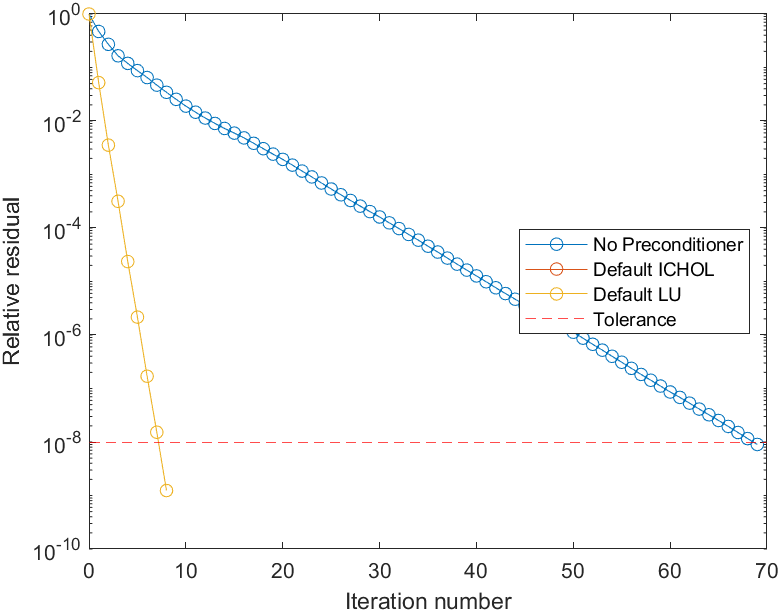
\includegraphics[scale=0.70]{img/thermomech/pcg}}
    \caption{История невязок методом pcg для матрицы Thermomech_dM}
    \label{fig:image_29}
\end{figure}

\begin{figure}[H]
    \renewcommand{\figurename}{Рисунок}
    \centering{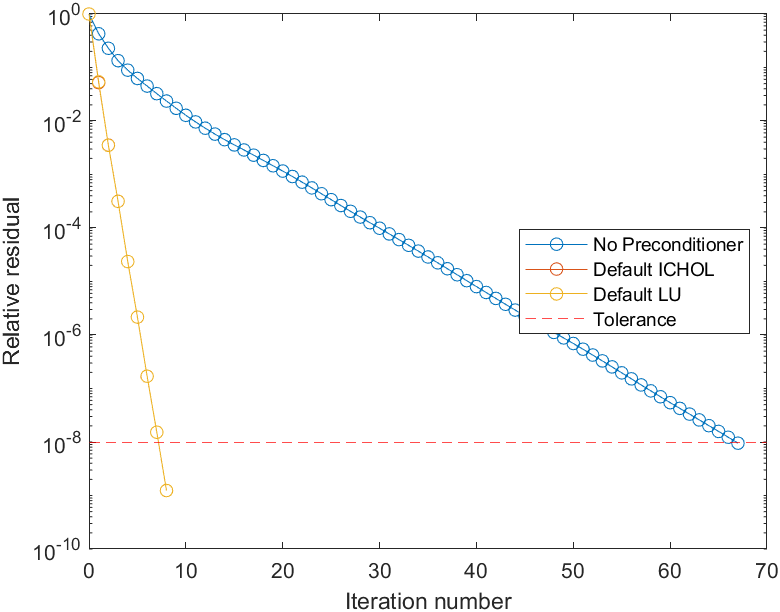
\includegraphics[scale=0.70]{img/thermomech/qmr}}
    \caption{История невязок методом qmr для матрицы Thermomech_dM}
    \label{fig:image_30}
\end{figure}

\begin{figure}[H]
    \renewcommand{\figurename}{Рисунок}
    \centering{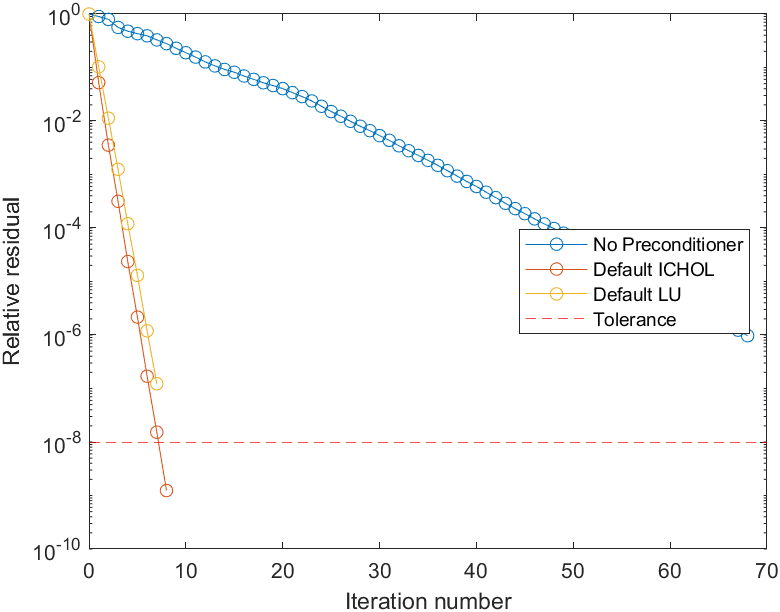
\includegraphics[scale=0.70]{img/thermomech/symmlq}}
    \caption{История невязок методом symmlq для матрицы Thermomech_dM}
    \label{fig:image_31}
\end{figure}

\begin{figure}[H]
    \renewcommand{\figurename}{Рисунок}
    \centering{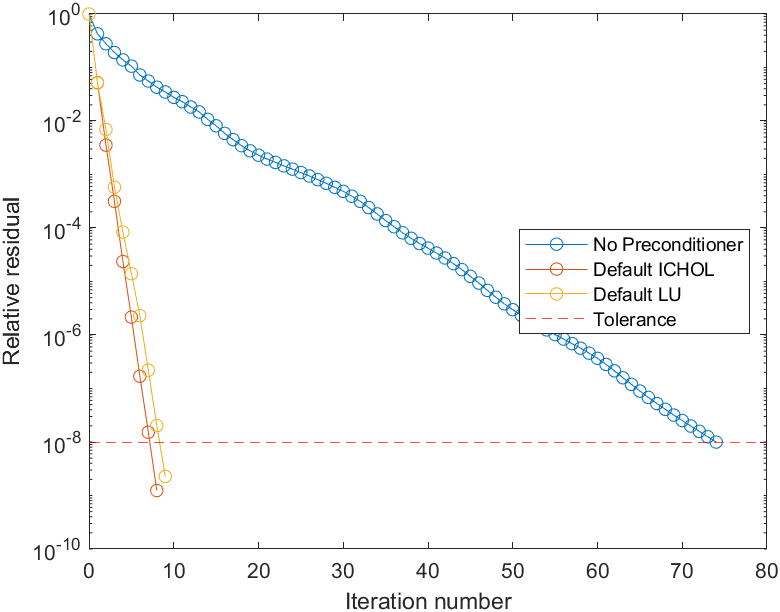
\includegraphics[scale=0.70]{img/thermomech/tfqmr}}
    \caption{История невязок методом tfqmr для матрицы Thermomech_dM}
    \label{fig:image_32}
\end{figure}